% The generic preamble
\documentclass[10pt,letterpaper,fleqn,titlepage]{article}

% Define packages to use
\usepackage{natbib}
\usepackage[dvips]{graphicx,color}
\usepackage{amsmath,amssymb}
\usepackage{bm}
\usepackage{caption}
\usepackage{xr}
\usepackage{ifthen}
\usepackage[dvipdfm,colorlinks,linkcolor=blue,citecolor=blue,urlcolor=blue]{hyperref}
\usepackage{fancybox}
\usepackage{textcomp}
\usepackage{alltt}
%\usepackage{floatflt}
%\usepackage{svn}


% Redefine default page
\setlength{\textheight}{9in}  % 1" above and below
\setlength{\textwidth}{6.75in}   % 0.5" left and right
\setlength{\oddsidemargin}{-0.25in}

% Redefine default paragraph
\setlength{\parindent}{0pt}
\setlength{\parskip}{1ex plus 0.5ex minus 0.2ex}

% Define caption width and default fonts
\setlength{\captionmargin}{0.5in}
\renewcommand{\captionfont}{\sffamily}
\renewcommand{\captionlabelfont}{\bfseries\sffamily}

% Define commands for super- and subscript in text mode
\newcommand{\superscript}[1]{\ensuremath{^\textrm{#1}}}
\newcommand{\subscript}[1]{\ensuremath{_\textrm{#1}}}

% Derived commands
\newcommand{\invcm}{\textrm{cm\superscript{-1}}}
\newcommand{\micron}{\ensuremath{\mu\textrm{m}}}

\newcommand{\df}{\ensuremath{\delta f}}
\newcommand{\Df}{\ensuremath{\Delta f}}
\newcommand{\dx}{\ensuremath{\delta x}}
\newcommand{\Dx}{\ensuremath{X_{max}}}
\newcommand{\Xeff}{\ensuremath{X_{eff}}}

\newcommand{\water}{\textrm{H\subscript{2}O}}
\newcommand{\carbondioxide}{\textrm{CO\subscript{2}}}
\newcommand{\ozone}{\textrm{O\subscript{3}}}

\newcommand{\taup}[1]{\ensuremath{\tau_{#1}}}
\newcommand{\efftaup}[1]{\ensuremath{\tau_{#1}^{*}}}

\newcommand{\textbfm}[1]{\boldmath\ensuremath{#1}\unboldmath}

\newcommand{\rb}[1]{\raisebox{1.5ex}[0pt]{#1}}

\newcommand{\f}[1]{\texttt{#1}}

% Define how equations are numbered
\numberwithin{equation}{section}
\numberwithin{figure}{section}
\numberwithin{table}{section}

% Define a command for title page author email footnote
\newcommand{\email}[1]
{%
  \renewcommand{\thefootnote}{\alph{footnote}}%
  \footnote{#1}
  \renewcommand{\thefootnote}{\arabic{footnote}}
}

% Define a command to print the Office Note subheading
\newcommand{\notesubheading}[1]
{%
  \ifthenelse{\equal{#1}{}}{}
  { {\Large\bfseries Office Note #1\par}%
    {\scriptsize \sc This is an unreviewed manuscript, primarily intended for informal}\\ 
    {\scriptsize \sc exchange of information among JCSDA researchers\par}%
  }
}

% Redefine the maketitle macro
\makeatletter
\def\docseries#1{\def\@docseries{#1}}
\def\docnumber#1{\def\@docnumber{#1}}
\renewcommand{\maketitle}
{%
  \thispagestyle{empty}
  \vspace*{1in}
  \begin{center}%
     \sffamily
     {\huge\bfseries Joint Center for Satellite Data Assimilation\par}%
     \notesubheading{\@docnumber}
  \end{center}
  \begin{flushleft}%
     \sffamily
     \vspace*{0.5in}
     {\Large\bfseries\ifthenelse{\equal{\@docseries}{}}{}{\@docseries: }\@title\par}%
     \medskip
     {\large\@author\par}%
     \medskip
     {\large\@date\par}%
     \bigskip\hrule\vspace*{2pc}%
  \end{flushleft}%
  \newpage
  \setcounter{footnote}{0}
}
\makeatother
\docseries{}
\docnumber{}


% Define a command for a DRAFT watermark
\usepackage{eso-pic}
\newcommand{\draftwatermark}
{
  \AddToShipoutPicture{%
    \definecolor{lightgray}{gray}{.85}
    \setlength{\unitlength}{1in}
    \put(2.5,3.5){%
      \rotatebox{45}{%
        \resizebox{4in}{1in}{%
          \textsf{\textcolor{lightgray}{DRAFT}}
        }
      }
    }
  }
}




% Include files
\includeonly{SRF_Data_Plots.app,Tfit_Data_Plots.app}

% Subversion keywords
\SVN $Date$
\SVN $Revision$

% Title info
\title{GMI GPM Spectral Response Function Processing}
\author{Paul van Delst\email{paul.vandelst@noaa.gov}\\NCEP/EMC/IMSG}
\date{\SVNDate ; rev\SVNRevision}
\docnumber{2}
\docseries{CRTM}


%-------------------------------------------------------------------------------
%                            Ze document begins...
%-------------------------------------------------------------------------------
\begin{document}
\maketitle

%\draftwatermark

% The front matter
%=================
\thispagestyle{empty}
\vspace*{10cm}
\begin{center}
  {\sffamily\Large\bfseries Change History}
  \begin{table}[htp]
    \centering
    \begin{tabular}{|p{2cm}|p{3cm}|p{8cm}|}
      \hline
      \sffamily\textbf{Date} & \sffamily\textbf{Author} & \sffamily\textbf{Change}\\
      \hline\hline
      2013-11-19 & Paul van Delst & Initial release.\\
      \hline
    \end{tabular}
  \end{table}
\end{center}
\clearpage
\pagestyle{fancy}
\fancyhead[LE,RO]{\sffamily \rightmark}
\fancyhead[LO,RE]{\sffamily \leftmark}
\pagenumbering{arabic}
\setcounter{page}{1}


% The main matter
%================

\section{Introduction}
%=====================
This document describes the pre-processing applied to the Global Precipitation Measurement (GPM) Microwave Imager (GMI) spectral response functions (SRFs), obtained from \cite{GMI_SRF_Data} and described in \citet{GMI_SER}, to prepare for use in the CRTM processing chain. The SRFs are used to generate channel central frequencies, as well as in the convolution of monochromatic quantities such as Planck radiances or line-by-line (LBL) model generated transmittances to produce such things as polychromatic correction coefficients and instrument resolution transmittances. The latter, for a diverse set of atmospheric profiles, are then regressed against a set of predictors to produce the fast transmittance model coefficients used by the CRTM.

The specification channel information is summarised in table \ref{tab:gmi_spectral_info}.
\begin{table}[htp]
  \centering
  \begin{tabular}{c c c c}
    \hline
    \sffamily{GMI}     & \sffamily{Centre Frequency} & \sffamily{Polarisation} & \sffamily{Passband width}\\
    \sffamily{Channel} & \sffamily{(GHz)} & & \sffamily{(MHz)}\\
    \hline\hline
     1 & 10.65 & V & 100 \\
     2 & 10.65 & H & 100 \\
     3 & 18.70 & V & 200 \\
     4 & 18.70 & H & 200 \\
     5 & 23.80 & V & 400 \\
     6 & 36.50 & V & 1000 \\
     7 & 36.50 & H & 1000 \\
     8 & 89.00 & V & 6000 \\
     9 & 89.00 & H & 6000 \\
    10 & 166.0 & V & 4000 \\
    11 & 166.0 & H & 4000 \\
    12 & 183.31$\pm$3.0 & V & 2000 \\
    13 & 183.31$\pm$7.0 & V & 2000 \\
    \hline
  \end{tabular}
  \caption{The GPM GMI spectral information.}
  \label{tab:gmi_spectral_info}
\end{table}

\subsection{Conversion from decibel to relative response}
%--------------------------------------------------------
All of the GMI response data were in units of decibels ($\phi_{dB}$). For use with the LBL model they were converted to a relative response ($\phi_{rel}$) using the following equation,
\begin{equation}
  \phi_{rel} = 10^{\displaystyle(\phi_{dB}-\max(\phi_{dB}))/10}
\end{equation} 


\subsection{Computation of the channel central frequency}
%--------------------------------------------------------
The computed GMI channel central frequencies, $\nu_0$, are the first moments of the defined SRF,
\begin{equation}
  \nu_0 = \frac{\displaystyle\int{\nu\:\phi_{rel}(\nu)\ud \nu}}{\displaystyle\int{\phi_{rel}(\nu)\ud \nu}}
\end{equation}
For multiple passband channels, each band is numerically integrated and summed to give the total. It should also be noted that all calculations (in the SRF processing, but also in the CRTM itself) are done in frequency units of cm\superscript{-1}. Conversion to units of GHz is done for display purposes only.


\subsection{Computation of polychromatic correction coefficients}
%----------------------------------------------------------------
In the CRTM, the conversion of \emph{channel resolution} radiances to brightness temperatures has to take the passband widths into account. For any channel, the regression relation to be solved is

\begin{equation}
  a_0 + a_1T + \ldots = \frac{\displaystyle k_1}{\displaystyle \ln\left[\frac{k_2}{R(T)}+1\right]} = Y(T)
\end{equation}
where
\begin{equation}
  \begin{array}{r@{\;=\;}l}
         T &\mbox{brightness temperature} \\
        a_j&\mbox{regression coefficients} \\
    k_1,k_2&\mbox{Planck coefficients} \\
       R(T)&\mbox{channel radiance} \\
       Y(T)&\mbox{``effective'' brightness temperature}
  \end{array}
\end{equation}
and the channel radiances used to determine the effective temperatures, $Y(T)$, are computed the usual way
\begin{equation}
  R(T) = \frac{\displaystyle\int{B(T,\nu)\:\phi_{rel}(\nu)\ud \nu}}{\displaystyle\int{\phi_{rel}(\nu)\ud \nu}}
\end{equation}
The quantity minimised to obtain the $a_j$ coefficients is
\begin{equation}
  \left[ \sum_{j=0}^{M}a_j T_{i} - Y(T_{i}) \right]^2 \quad\mbox{for}\quad T_i = 150K, \ldots, 340K \;\mbox{ in 5K steps.}
\end{equation}
Currently the number of coefficients is fixed at two (i.e. $M=1$).



\newpage
\section{Summary}
%================

\subsection{Selected testing temperatures}
%-----------------------------------------
Three common temperatures were available for all the received data files. They appear to correspond to the ``usual'' nominal, low, and high operating temperatures; in this case 25\textdegree{}C, -10\textdegree{}C, and 45\textdegree{}C respectively. The actual testing temperatures specified in the supplied datafiles for each channel are shown in table \ref{tab:gmi_test_temperatures}.

\begin{table}[htp]
  \centering
  \begin{tabular}{c *{3}{c r@{.}l}}
    \hline
    \sffamily{GMI} & & \multicolumn{2}{c}{\sffamily{T\subscript{\sffamily{NOM}}}} & & \multicolumn{2}{c}{\sffamily{T\subscript{\sffamily{LO}}}} & & \multicolumn{2}{c}{\sffamily{T\subscript{\sffamily{HI}}}}\\
    \sffamily{Channel} & & \multicolumn{2}{c}{\sffamily{(\textdegree{}C)}} & & \multicolumn{2}{c}{\sffamily{(\textdegree{}C)}} & & \multicolumn{2}{c}{\sffamily{(\textdegree{}C)}}  \\
    \hline\hline
    1  & & 22&9 & & -10&7 & & 45&0  \\
    2  & & 22&9 & & -10&7 & & 45&0  \\
    3  & & 25&0 & & -10&2 & & 45&05 \\
    4  & & 25&0 & & -10&2 & & 45&0  \\ 
    5  & & 25&0 & & -10&2 & & 45&0  \\
    6  & & 26&0 & & -11&0 & & 45&0  \\
    7  & & 26&0 & & -10&0 & & 44&0  \\
    8  & & 25&0 & & -10&0 & & 45&0  \\
    9  & & 25&0 & & -10&0 & & 45&0  \\
    10 & & 25&8 & & -10&7 & & 45&4  \\
    11 & & 25&8 & & -10&7 & & 45&4  \\
    12 & & 25&4 & &  -9&7 & & 45&9  \\
    13 & & 25&4 & &  -9&7 & & 45&9  \\
    \hline
  \end{tabular}
  \caption{The low, nominal, and high temperatures selected for each GMI channel.}
  \label{tab:gmi_test_temperatures}
\end{table}

All of the GMI SRFs had a threshold of 0.01\% applied to minimise LBL model computation time (see section \ref{sec:threshold_impact}). Plots of the SRFs data used for each test temperature and channel are shown in appendix \ref{app.srf_data_plots}.


\subsection{SRF processing}
%--------------------------
The following tables list the computed central frequencies and polychromatic correction coefficients for the three test temperatures. The temperature fit residuals for each temperature and each channel are shown in appendix \ref{app.tfit_data_plots}.

\subsubsection{T\subscript{NOM} results}
%.......................................

\begin{table}[htp]
  \centering
  \begin{tabular}{c *{3}{c r@{.}l}}
    \hline
    \sffamily{GMI} & & \multicolumn{2}{c}{$f_0$} & & \multicolumn{2}{c}{$a_0$ (offset)} & & \multicolumn{2}{c}{$a_1$ (slope)} \\
    \sffamily{Channel} & & \multicolumn{2}{c}{\sffamily{(GHz)}} & & \multicolumn{2}{c}{\sffamily{(K)}} & & \multicolumn{2}{c}{\sffamily{(K/K)}}  \\
    \hline\hline

    1  & &  10&647550 & & -0&00000524 & & 1&00000685 \\
    2  & &  10&645034 & & -0&00000509 & & 1&00000666 \\
    3  & &  18&688988 & & -0&00001181 & & 1&00000881 \\
    4  & &  18&687572 & & -0&00001193 & & 1&00000890 \\
    5  & &  23&810267 & & -0&00003320 & & 1&00001945 \\
    6  & &  36&625238 & & -0&00007538 & & 1&00002876 \\
    7  & &  36&649512 & & -0&00007591 & & 1&00002895 \\
    8  & &  89&034827 & & -0&00272505 & & 1&00043150 \\
    9  & &  88&957954 & & -0&00279814 & & 1&00044324 \\
    10 & & 166&090577 & & -0&00064672 & & 1&00005557 \\
    11 & & 166&118649 & & -0&00065959 & & 1&00005667 \\
    12 & & 183&253683 & & -0&00346990 & & 1&00027083 \\
    13 & & 182&828245 & & -0&01864121 & & 1&00145602 \\
    \hline
  \end{tabular}
  \caption{The computed GMI channel central frequencies and polychromatic correction coefficients for the T\subscript{\sffamily{NOM}} SRF dataset.}
  \label{tab:gmi_TNOM_results}
\end{table}


\subsubsection{T\subscript{LO} results}
%......................................

\begin{table}[H]
  \centering
  \begin{tabular}{c *{3}{c r@{.}l}}
    \hline
    \sffamily{GMI} & & \multicolumn{2}{c}{$f_0$} & & \multicolumn{2}{c}{$a_0$ (offset)} & & \multicolumn{2}{c}{$a_1$ (slope)} \\
    \sffamily{Channel} & & \multicolumn{2}{c}{\sffamily{(GHz)}} & & \multicolumn{2}{c}{\sffamily{(K)}} & & \multicolumn{2}{c}{\sffamily{(K/K)}}  \\
    \hline\hline

    1  & &  10&648052 & & -0&00000524 & & 1&00000684 \\
    2  & &  10&645618 & & -0&00000511 & & 1&00000668 \\
    3  & &  18&689398 & & -0&00001190 & & 1&00000888 \\
    4  & &  18&686355 & & -0&00001200 & & 1&00000895 \\
    5  & &  23&811794 & & -0&00003356 & & 1&00001965 \\
    6  & &  36&628822 & & -0&00007432 & & 1&00002835 \\
    7  & &  36&653028 & & -0&00007604 & & 1&00002900 \\
    8  & &  89&036071 & & -0&00273565 & & 1&00043319 \\
    9  & &  88&931517 & & -0&00279681 & & 1&00044312 \\
    10 & & 166&058309 & & -0&00065352 & & 1&00005616 \\
    11 & & 166&109436 & & -0&00066650 & & 1&00005727 \\
    12 & & 183&239186 & & -0&00347025 & & 1&00027087 \\
    13 & & 182&768792 & & -0&01874660 & & 1&00146441 \\
    \hline
  \end{tabular}
  \caption{The computed GMI channel central frequencies and polychromatic correction coefficients for the T\subscript{\sffamily{LO}} SRF dataset.}
  \label{tab:gmi_TLO_results}
\end{table}


\subsubsection{T\subscript{HI} results}
%......................................

\begin{table}[H]
  \centering
  \begin{tabular}{c *{3}{c r@{.}l}}
    \hline
    \sffamily{GMI} & & \multicolumn{2}{c}{$f_0$} & & \multicolumn{2}{c}{$a_0$ (offset)} & & \multicolumn{2}{c}{$a_1$ (slope)} \\
    \sffamily{Channel} & & \multicolumn{2}{c}{\sffamily{(GHz)}} & & \multicolumn{2}{c}{\sffamily{(K)}} & & \multicolumn{2}{c}{\sffamily{(K/K)}}  \\
    \hline\hline

    1  & &  10&647713 & & -0&00000522 & & 1&00000683 \\
    2  & &  10&645221 & & -0&00000507 & & 1&00000663 \\
    3  & &  18&688659 & & -0&00001180 & & 1&00000880 \\
    4  & &  18&686505 & & -0&00001183 & & 1&00000882 \\
    5  & &  23&810498 & & -0&00003322 & & 1&00001946 \\
    6  & &  36&625805 & & -0&00007676 & & 1&00002928 \\
    7  & &  36&648478 & & -0&00007609 & & 1&00002902 \\
    8  & &  89&034402 & & -0&00271545 & & 1&00042997 \\
    9  & &  88&945400 & & -0&00280271 & & 1&00044399 \\
    10 & & 166&094910 & & -0&00064524 & & 1&00005544 \\
    11 & & 166&132543 & & -0&00065699 & & 1&00005645 \\
    12 & & 183&262584 & & -0&00346862 & & 1&00027073 \\
    13 & & 182&821958 & & -0&01867263 & & 1&00145848 \\
    \hline
  \end{tabular}
  \caption{The computed GMI channel central frequencies and polychromatic correction coefficients for the T\subscript{\sffamily{HI}} SRF dataset.}
  \label{tab:gmi_THI_results}
\end{table}



\newpage
\section{Impact of response threshold on convolved radiances}
%============================================================
\label{sec:threshold_impact}
All of the GMI SRFs appear similarly to that shown in figure \ref{fig:gmi_gpm.no_threshold.channel1} where there is a wide spectral region containing data that does not contribute significantly to the channel response. To minimise line-by-line calculations, the SRFs are spectrally ``trimmed'' by applying a response threshold; that is, when the SRF magnitudes drop below a certain value the data are discarded.

\begin{figure}[H]
  \centering
  \includegraphics[scale=0.8]{graphics/gmi_gpm.no_threshold.channel1.eps}
  \caption{GPM GMI channel 1 spectral response function (SRF) at T $\sim$ 25C.}
  \label{fig:gmi_gpm.no_threshold.channel1}
\end{figure}

The thresholding methodology used in the CRTM SRF processing applies a response threshold whilst scanning through the SRF in four directions:
\begin{itemize}
  \item Increasing from the lowest frequency to that for the maximum SRF value. The first point at which the SRF magnitude is \emph{above} the threshold is labeled as the \textbf{outer low-frequency cutoff} value.
  \item Decreasing from the highest frequency to that for the maximum SRF value. The first point at which the SRF magnitude is \emph{above} the threshold is labeled as the \textbf{outer high-frequency cutoff} value.
  \item Decreasing from the frequency of the maximum SRF value to the lowest frequency. The previous point to the first point for which the SRF magnitude is \emph{below} the threshold is labeled as the \textbf{inner low-frequency cutoff} value.
  \item Increasing from the frequency of the maximum SRF value to the highest frequency. The previous point to the first point for which the SRF magnitude is \emph{below} the threshold is labeled as the \textbf{inner high-frequency cutoff} value.
\end{itemize}
For a suitably chosen response threshold, the inner and outer cutoff points on either side of the SRF itself should coincide. The operative phrase in the previous sentence is ``suitably chosen''. We do not want to discard SRF data that is significant in terms of channel response.

Inspection of the GMI SRFs led to a response cutoff of $10^{-4}$ (0.01\%)being chosen\footnote{Note that the ``standard'' response thresholds applied to infrared and visible channels are 0.1 and 1\% respectively}. This results in SRFs like those shown in figure \ref{fig:gmi_gpm.with_threshold.channel1} for channel 1 and \ref{fig:gmi_gpm.with_threshold.channel11} for channel 11.

\begin{figure}[H]
  \centering
  \includegraphics[scale=0.8]{graphics/gmi_gpm.with_threshold.channel1.eps}
  \caption{GPM GMI channel 1 spectral response function (SRF) at T $\sim$ 25C showing the original (red) and processed (blue) SRF with a response threshold of $10^{-4}$ applied.}
  \label{fig:gmi_gpm.with_threshold.channel1}
\end{figure}

\begin{figure}[H]
  \centering
  \includegraphics[scale=0.8]{graphics/gmi_gpm.with_threshold.channel11.eps}
  \caption{GPM GMI channel 11 double-passband spectral response function (SRF) at T $\sim$ 25C showing the original (red) and processed (blue) SRF with a response threshold of $10^{-4}$ applied.}
  \label{fig:gmi_gpm.with_threshold.channel11}
\end{figure}


To determine if there was any significant difference introduced by applying the $10^{-4}$ response threshold to the GMI SRFs, both sets of data (original and thresholded) were convolved with LBL-model generated radiances.

MonoRTM (\cite{MonoRTM1}, \cite{MonoRTM2}) was used with the ECMWF83 atmospheric profile dataset to generate radiance spectra. The radiance spectra were convoled with the SRFs to yield channel resolution radiances which were then converted to brightness temperatures for each SRF set. The statistics of the brightness temperature differences are shown in figure \ref{fig:TNOM_threshold_dTb_stats}. The largest individual differences are of the order of $10^{-4}$K so using the threshold SRFs will not introduce any significant bias into the channel radiances. The LBL model computation time using the threshold SRFs was 50\% faster. 

\begin{figure}[H]
  \centering
  \includegraphics[scale=0.75]{graphics/TNOM_threshold_dTb_stats.eps}
  \caption{Statistics of the brightness temperature differences when a response threshold of $10^{-4}$ is applied to the GMI channel SRFs. The calculations used MonoRTM v4.0 and the ECMWF83 profile dataset with a surface emissivity of 0.6.}
  \label{fig:TNOM_threshold_dTb_stats}
\end{figure}


\newpage
\section{Impact of SRF measurement temperature on convolved radiances}
%=====================================================================
Similarly to the procedure used to determine the impact of a response threshold, to quantify the differences due to the SRF measurement temperature all three sets of SRFs ($T_{NOM}$, $T_{LO}$, $T_{HI}$) -- with the $10^{-4}$ response threshold applied -- were convolved with LBL-model generated radiances (using the same LBL model and atmospheric profile set described in section \ref{sec:threshold_impact}). See appendix \ref{app.srf_data_plots} for plots of the three sets of GMI SRF data.

The statistics of the brightness temperature differences due to the differences in the $T_{LO/HI}$ SRF data compared to the $T_{NOM}$ SRFs are shown in figure \ref{fig:TLO-THI_dTb_stats}. Here we see the average differences are around $10^{-2}$K with the largest individual differences of the order of $10^{-1}$K.

\begin{figure}[H]
  \centering
  \includegraphics[scale=0.75]{graphics/TLO-THI_dTb_stats.eps}
  \caption{Statistics of the brightness temperature differences due to the differences in the $T_{LO/HI}$ SRF data compared to the $T_{NOM}$ SRFs. All three SRF sets have a response threshold of $10^{-4}$ applied. The calculations used MonoRTM v4.0 and the ECMWF83 profile dataset with a surface emissivity of 0.6.}
  \label{fig:TLO-THI_dTb_stats}
\end{figure}


% The references section
%=======================
\clearpage
\bibliographystyle{plainnat}
\bibliography{bibliography}


% The appendices section
%=======================
\begin{appendix}
  \section{GMI SRF Data Plots}
%===========================
\label{app.srf_data_plots}
\newpage

\addcontentsline{toc}{subsection}{Channel 1}
\begin{figure}[htp]
  \centering
  \begin{tabular}{c c}
    \includegraphics[scale=0.3]{graphics/lin/gmi_gpm-1.eps} &
    \includegraphics[scale=0.3]{graphics/log/gmi_gpm-1.eps}
  \end{tabular}
  \caption{GMI channel 1 responses for the three test temperatures: $T_{NOM}$ (25\textdegree{}C), $T_{LO}$ (-10\textdegree{}C), and $T_{HI}$ (45\textdegree{}C). Vertical dashed lines are the locations of the computed central frequencies. \textbf{(Left)} Linear y-axis. \textbf{(Right)} Base-10 logarithmic y-axis.}
  \label{fig:ch1_response}
\end{figure}

\addcontentsline{toc}{subsection}{Channel 2}
\begin{figure}[htp]
  \centering
  \begin{tabular}{c c}
    \includegraphics[scale=0.3]{graphics/lin/gmi_gpm-2.eps} &
    \includegraphics[scale=0.3]{graphics/log/gmi_gpm-2.eps}
  \end{tabular}
  \caption{GMI channel 2 responses for the three test temperatures: $T_{NOM}$ (25\textdegree{}C), $T_{LO}$ (-10\textdegree{}C), and $T_{HI}$ (45\textdegree{}C). Vertical dashed lines are the locations of the computed central frequencies. \textbf{(Left)} Linear y-axis. \textbf{(Right)} Base-10 logarithmic y-axis.}
  \label{fig:ch2_response}
\end{figure}

\addcontentsline{toc}{subsection}{Channel 3}
\begin{figure}[htp]
  \centering
  \begin{tabular}{c c}
    \includegraphics[scale=0.3]{graphics/lin/gmi_gpm-3.eps} &
    \includegraphics[scale=0.3]{graphics/log/gmi_gpm-3.eps}
  \end{tabular}
  \caption{GMI channel 3 responses for the three test temperatures: $T_{NOM}$ (25\textdegree{}C), $T_{LO}$ (-10\textdegree{}C), and $T_{HI}$ (45\textdegree{}C). Vertical dashed lines are the locations of the computed central frequencies. \textbf{(Left)} Linear y-axis. \textbf{(Right)} Base-10 logarithmic y-axis.}
  \label{fig:ch3_response}
\end{figure}

\addcontentsline{toc}{subsection}{Channel 4}
\begin{figure}[htp]
  \centering
  \begin{tabular}{c c}
    \includegraphics[scale=0.3]{graphics/lin/gmi_gpm-4.eps} &
    \includegraphics[scale=0.3]{graphics/log/gmi_gpm-4.eps}
  \end{tabular}
  \caption{GMI channel 4 responses for the three test temperatures: $T_{NOM}$ (25\textdegree{}C), $T_{LO}$ (-10\textdegree{}C), and $T_{HI}$ (45\textdegree{}C). Vertical dashed lines are the locations of the computed central frequencies. \textbf{(Left)} Linear y-axis. \textbf{(Right)} Base-10 logarithmic y-axis.}
  \label{fig:ch4_response}
\end{figure}

\addcontentsline{toc}{subsection}{Channel 5}
\begin{figure}[htp]
  \centering
  \begin{tabular}{c c}
    \includegraphics[scale=0.3]{graphics/lin/gmi_gpm-5.eps} &
    \includegraphics[scale=0.3]{graphics/log/gmi_gpm-5.eps}
  \end{tabular}
  \caption{GMI channel 5 responses for the three test temperatures: $T_{NOM}$ (25\textdegree{}C), $T_{LO}$ (-10\textdegree{}C), and $T_{HI}$ (45\textdegree{}C). Vertical dashed lines are the locations of the computed central frequencies. \textbf{(Left)} Linear y-axis. \textbf{(Right)} Base-10 logarithmic y-axis.}
  \label{fig:ch5_response}
\end{figure}

\addcontentsline{toc}{subsection}{Channel 6}
\begin{figure}[htp]
  \centering
  \begin{tabular}{c c}
    \includegraphics[scale=0.3]{graphics/lin/gmi_gpm-6.eps} &
    \includegraphics[scale=0.3]{graphics/log/gmi_gpm-6.eps}
  \end{tabular}
  \caption{GMI channel 6 responses for the three test temperatures: $T_{NOM}$ (25\textdegree{}C), $T_{LO}$ (-10\textdegree{}C), and $T_{HI}$ (45\textdegree{}C). Vertical dashed lines are the locations of the computed central frequencies. \textbf{(Left)} Linear y-axis. \textbf{(Right)} Base-10 logarithmic y-axis.}
  \label{fig:ch6_response}
\end{figure}

\addcontentsline{toc}{subsection}{Channel 7}
\begin{figure}[htp]
  \centering
  \begin{tabular}{c c}
    \includegraphics[scale=0.3]{graphics/lin/gmi_gpm-7.eps} &
    \includegraphics[scale=0.3]{graphics/log/gmi_gpm-7.eps}
  \end{tabular}
  \caption{GMI channel 7 responses for the three test temperatures: $T_{NOM}$ (25\textdegree{}C), $T_{LO}$ (-10\textdegree{}C), and $T_{HI}$ (45\textdegree{}C). Vertical dashed lines are the locations of the computed central frequencies. \textbf{(Left)} Linear y-axis. \textbf{(Right)} Base-10 logarithmic y-axis.}
  \label{fig:ch7_response}
\end{figure}

\addcontentsline{toc}{subsection}{Channel 8}
\begin{figure}[htp]
  \centering
  \begin{tabular}{c c}
    \includegraphics[scale=0.3]{graphics/lin/gmi_gpm-8.eps} &
    \includegraphics[scale=0.3]{graphics/log/gmi_gpm-8.eps}
  \end{tabular}
  \caption{GMI channel 8 responses for the three test temperatures: $T_{NOM}$ (25\textdegree{}C), $T_{LO}$ (-10\textdegree{}C), and $T_{HI}$ (45\textdegree{}C). \textbf{(Left)} Linear y-axis. \textbf{(Right)} Base-10 logarithmic y-axis.}
  \label{fig:ch8_response}
\end{figure}

\addcontentsline{toc}{subsection}{Channel 9}
\begin{figure}[htp]
  \centering
  \begin{tabular}{c c}
    \includegraphics[scale=0.3]{graphics/lin/gmi_gpm-9.eps} &
    \includegraphics[scale=0.3]{graphics/log/gmi_gpm-9.eps}
  \end{tabular}
  \caption{GMI channel 9 responses for the three test temperatures: $T_{NOM}$ (25\textdegree{}C), $T_{LO}$ (-10\textdegree{}C), and $T_{HI}$ (45\textdegree{}C). \textbf{(Left)} Linear y-axis. \textbf{(Right)} Base-10 logarithmic y-axis.}
  \label{fig:ch9_response}
\end{figure}

\addcontentsline{toc}{subsection}{Channel 10}
\begin{figure}[htp]
  \centering
  \begin{tabular}{c c}
    \includegraphics[scale=0.3]{graphics/lin/gmi_gpm-10.eps} &
    \includegraphics[scale=0.3]{graphics/log/gmi_gpm-10.eps}
  \end{tabular}
  \caption{GMI channel 10 responses for the three test temperatures: $T_{NOM}$ (25\textdegree{}C), $T_{LO}$ (-10\textdegree{}C), and $T_{HI}$ (45\textdegree{}C). \textbf{(Left)} Linear y-axis. \textbf{(Right)} Base-10 logarithmic y-axis.}
  \label{fig:ch10_response}
\end{figure}

\addcontentsline{toc}{subsection}{Channel 11}
\begin{figure}[htp]
  \centering
  \begin{tabular}{c c}
    \includegraphics[scale=0.3]{graphics/lin/gmi_gpm-11.eps} &
    \includegraphics[scale=0.3]{graphics/log/gmi_gpm-11.eps}
  \end{tabular}
  \caption{GMI channel 11 responses for the three test temperatures: $T_{NOM}$ (25\textdegree{}C), $T_{LO}$ (-10\textdegree{}C), and $T_{HI}$ (45\textdegree{}C). \textbf{(Left)} Linear y-axis. \textbf{(Right)} Base-10 logarithmic y-axis.}
  \label{fig:ch11_response}
\end{figure}

\addcontentsline{toc}{subsection}{Channel 12}
\begin{figure}[htp]
  \centering
  \begin{tabular}{c c}
    \includegraphics[scale=0.3]{graphics/lin/gmi_gpm-12.eps} &
    \includegraphics[scale=0.3]{graphics/log/gmi_gpm-12.eps}
  \end{tabular}
  \caption{GMI channel 12 responses for the three test temperatures: $T_{NOM}$ (25\textdegree{}C), $T_{LO}$ (-10\textdegree{}C), and $T_{HI}$ (45\textdegree{}C). \textbf{(Left)} Linear y-axis. \textbf{(Right)} Base-10 logarithmic y-axis.}
  \label{fig:ch12_response}
\end{figure}

\addcontentsline{toc}{subsection}{Channel 13}
\begin{figure}[htp]
  \centering
  \begin{tabular}{c c}
    \includegraphics[scale=0.3]{graphics/lin/gmi_gpm-13.eps} &
    \includegraphics[scale=0.3]{graphics/log/gmi_gpm-13.eps}
  \end{tabular}
  \caption{GMI channel 13 responses for the three test temperatures: $T_{NOM}$ (25\textdegree{}C), $T_{LO}$ (-10\textdegree{}C), and $T_{HI}$ (45\textdegree{}C). \textbf{(Left)} Linear y-axis. \textbf{(Right)} Base-10 logarithmic y-axis.}
  \label{fig:ch13_response}
\end{figure}


  \section{Polychromatic Correction Temperature Fit Residual Data Plots}
%=====================================================================
\label{app.tfit_data_plots}
%\newpage

\addcontentsline{toc}{subsection}{Channels 1-6}
\begin{figure}[H]
  \centering
  \begin{tabular}{c c}
    \includegraphics[scale=0.35]{graphics/tfit/gmi_gpm-1.tfit.eps} &
    \includegraphics[scale=0.35]{graphics/tfit/gmi_gpm-2.tfit.eps} \\\\
    \includegraphics[scale=0.35]{graphics/tfit/gmi_gpm-3.tfit.eps} &
    \includegraphics[scale=0.35]{graphics/tfit/gmi_gpm-4.tfit.eps} \\\\
    \includegraphics[scale=0.35]{graphics/tfit/gmi_gpm-5.tfit.eps} &
    \includegraphics[scale=0.35]{graphics/tfit/gmi_gpm-6.tfit.eps} \\
  \end{tabular}
  \caption{GMI channels 1-6 polychromatic correction temperature fit residuals for the three test temperatures: $T_{NOM}$ (25\textdegree{}C), $T_{LO}$ (-10\textdegree{}C), and $T_{HI}$ (45\textdegree{}C).}
  \label{fig:ch1-6_tfit}
\end{figure}

\addcontentsline{toc}{subsection}{Channels 7-12}
\begin{figure}[H]
  \centering
  \begin{tabular}{c c}
    \includegraphics[scale=0.35]{graphics/tfit/gmi_gpm-7.tfit.eps} &
    \includegraphics[scale=0.35]{graphics/tfit/gmi_gpm-8.tfit.eps} \\\\
    \includegraphics[scale=0.35]{graphics/tfit/gmi_gpm-9.tfit.eps} &
    \includegraphics[scale=0.35]{graphics/tfit/gmi_gpm-10.tfit.eps} \\\\
    \includegraphics[scale=0.35]{graphics/tfit/gmi_gpm-11.tfit.eps} &
    \includegraphics[scale=0.35]{graphics/tfit/gmi_gpm-12.tfit.eps} \\
  \end{tabular}
  \caption{GMI channels 7-12 polychromatic correction temperature fit residuals for the three test temperatures: $T_{NOM}$ (25\textdegree{}C), $T_{LO}$ (-10\textdegree{}C), and $T_{HI}$ (45\textdegree{}C).}
  \label{fig:ch7-12_tfit}
\end{figure}

\addcontentsline{toc}{subsection}{Channel 13}
\begin{figure}[H]
  \centering
  \includegraphics[scale=0.35]{graphics/tfit/gmi_gpm-13.tfit.eps}
  \caption{GMI channel 13 polychromatic correction temperature fit residuals for the three test temperatures: $T_{NOM}$ (25\textdegree{}C), $T_{LO}$ (-10\textdegree{}C), and $T_{HI}$ (45\textdegree{}C).}
  \label{fig:ch13_tfit}
\end{figure}


\end{appendix}

\end{document}

